\documentclass{sugconf}

% Change these 5 lines for your paper content
\sugconfsubject{Title for SAS Global Forum 2021 Sample Paper}
\sugconfpapernumber{Paper 0000-2021 (if SAS author use SAS0000-2021)}
\sugconfkeywords{SAS, Global Form, Template}
\title{Title for SAS Global Forum 2021 Sample Paper}
\author{Author 1 name, ABC Corporation; Author 2 name, DEF Corporation; Author 3 name, GHJ University}

% Don't touch these settings unless you know what you are doing
\makeatletter
\usepackage[
    bookmarks = false
    ,pdfauthor = {\@author}
    ,pdfcreator = { pdfLaTeX and sufconf.cls }
    ,pdfstartview = FitBH
    ,pdftitle = {\@title}
]{hyperref}\makeatother
\pdfcompresslevel=9
\pdfoutput=1
\usepackage{etoolbox}
\patchcmd{\thebibliography}{\section*{\refname}}{}{}{}
% End don't touch section

\begin{document}

\begin{abstract}
    This paragraph uses the PaperBody style, which uses the Verdana font, not the Arial font.
\end{abstract}

\section{Introduction}

This paragraph uses the PaperBody style, which uses the Verdana font, not the Arial font.

\section{First Main Topic}

This is a main topic in the body of the paper. This paragraph uses the PaperBody style, which uses the Verdana font, not the Arial font.
If you need to include source code, introduce it with a sentence that ends with a colon:

\begin{verbatim}
    proc ds2;
    data _null_; 
      method init(); 
        dcl varchar(16) str; 
        str = 'Hello World!'; 
        put str; 
      end;
    enddata;
    run;
    quit;
\end{verbatim}

Figure 1 is a sample figure.

\begin{figure}[!ht]
    \centering
    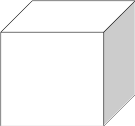
\includegraphics{figure1}
    \caption[Figure 1 is a sample figure]
    {Figure 1 is a sample figure}
\end{figure}

\subsection{Subhead A Level}

This is a subtopic of a main topic. This paragraph uses the PaperBody style, which uses the Verdana font, not the Arial font.

\begin{tabular}[t]{l l}
    \hline
    SAS Variable Format & DB2 Data Type \\
    \hline\hline
    \$$w.$  & CHARACTER \\
    CHAR$w.$ &   \\
    \hline
    any date format & DATE \\
    \hline
\end{tabular}

Table 1. DBLOAD Procedure: Default DB2 Data Types for SAS Variable Formats 

\section{Second Main Topic}

This is a main topic in the paper. This paragraph uses the PaperBody style, which uses the Verdana font, not the Arial font.

\begin{enumerate}
    \item This is a sample numbered or ordered list item. This is list item text. This is list item text. This is list item text. 
    \item This is a sample numbered or ordered list item. This is list item text.
\end{enumerate}

  This is another sample paragraph. This paragraph uses the PaperBody style, which uses the Verdana font, not the Arial font.

\begin{itemize}
    \item This is a sample bulleted list item. This is list item text. This is list item text. This is list item text. This is list item text.
    \item This is a sample bulleted list item. This is list item text. 
\end{itemize}

This is a continuation of the body of the paper—after an unordered list. This paragraph uses the PaperBody style, which uses the Verdana font, not the Arial font.

Display 1 is sample display or screen capture. 

\begin{figure}[!ht]
    \centering
    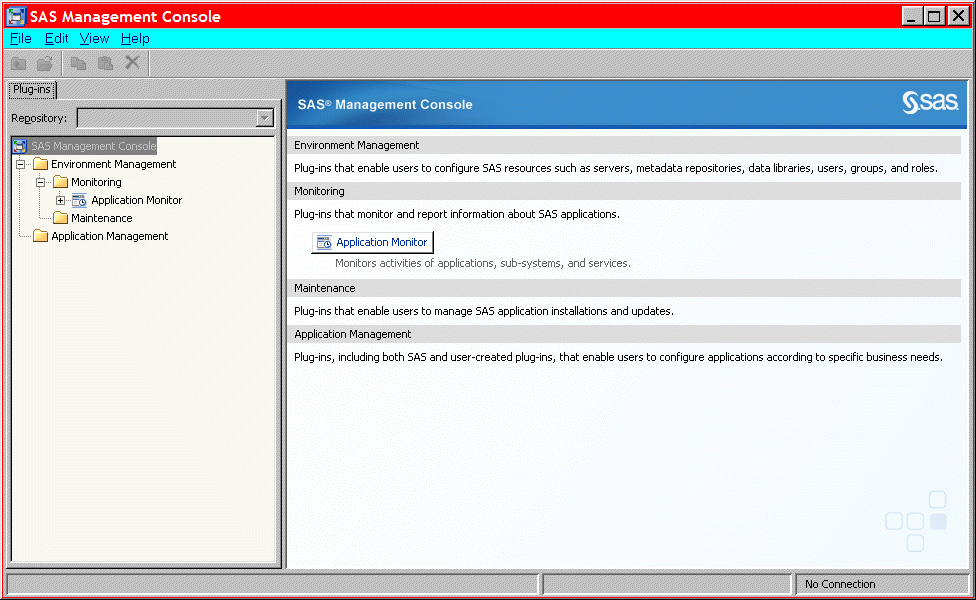
\includegraphics[width=\textwidth]{display1}
    {Former Main Interface for SAS Management Console}
\end{figure}

\subsection{Subhead A Level }

This paragraph uses the PaperBody style, which uses the Verdana font, not the Arial font.

\begin{verbatim}
    CREATE TABLE ALLACCTX(SourceSystem varchar(4),
    cctnum numeric(18,5) CONSTRAINT "ALLACCT_PK" PRIMARY KEY,
    ccttype numeric(18,5),balance numeric(18,5),clientid numeric(18,5),
    losedate date,opendate date,primary_cd numeric(18,5),status varchar(1))
\end{verbatim}

Output 1 shows an example of how to present output.

\subsubsection{Subhead B Level}

This is a subtopic of a subtopic. This paragraph uses the PaperBody style, which uses the Verdana font, not the Arial font.

\paragraph{Subhead C level}

This paragraph uses the PaperBody style, which uses the Verdana font, not the Arial font. 

\section{Conclusion}

This paragraph uses the PaperBody style, which uses the Verdana font, not the Arial font.

\section{References}

\nocite{*}
\bibliographystyle{acm}
\bibliography{biblio}

\section{Acknowledgements}

This is the text for the acknowledgments. This paragraph uses the PaperBody style, which uses the Verdana font, not the Arial font.

\section{Recommended Reading}

\begin{itemize}
    \item Base SAS\textregistered\xspace Procedures Guide 
    \item SAS\textregistered\xspace For Dummies\textregistered
\end{itemize}

\section{Contact Information}

Your comments and questions are valued and encouraged. Contact the author at:

\begin{tabular}[t]{l}
    Name  \\
    Enterprise (optional)  \\
    Phone (optional)  \\
    E-mail  \\ 
    Web (optional)  \\
\end{tabular}

\SASisRegisteredTrademark

\OtherTrademarks

\end{document}